\documentclass[11pt, norsk]{article}
%\usepackage[latin1]{inputenc}
\usepackage[T1]{fontenc}
\usepackage[utf8]{inputenc}
\usepackage[norsk]{babel}   % S P R A A K


% \usepackage{graphicx}    % postscript graphics
\usepackage{amssymb, amsmath, amsthm, amssymb} % symboler, osv
\usepackage{mathrsfs}
\usepackage{url}
\usepackage{thmtools}
\usepackage{enumerate}  % lister $  
\usepackage{float}
\usepackage{tikz}
\usetikzlibrary{calc}
\usepackage{tikz-3dplot}
\usepackage{subcaption}
\usepackage[all]{xy}   % for comm.diagram
\usepackage{wrapfig} % for float right
\usepackage{hyperref}
\usepackage{mystyle} % stilfilen      


\begin{document}
\title{Oppgaver MAT2500}
\author{Fredrik Meyer}
\maketitle 

\begin{oppg}
  La $ABCD$ og $A'BC'D'$ være to parallellogrammer med felles vinkel $\angle ABC= \angle A'BC'$. Vis at linjene gjennom $DD'$, $A'C$ og $AC'$ er konkurrente.
\end{oppg}
\begin{losn}
Det er essensielt sett to måter å løse denne oppgaven på. Den ene måten er algebraisk, og den andre er geometrisk. Vi tar den algebraiske først.

Vi skal studere ligningene til de forskjellige linjene, og vise at et punkt $X$ som ligger på linjen $AC'$ og på linjen $A'C$ også må ligge på $DD'$. 

Vi skal bruke vektornotasjon og vektorsummering. For at ting skal bli enkelt, antar vi at $B = \vec O$, origo.

Vi skal bruke en notasjon: Om $\vec V = (v,w)$, la $V^\perp$ betegne $(w,-v)$. Dette er da en vektor ortogonal med $\vec V$. Legg merke til at $(\vec V + \vec W)^\perp = \vec V^\perp + \vec W^\perp$. 

Da er ligningen for linjen $AC'$ gitt ved
\begin{equation}
\label{eq1}
(\vec {A'} - \vec{C})^\perp \cdot \vec X + \vec{A'} \cdot \vec C^\perp = 0
\end{equation}
Hvorfor er dette sant? Ligningen er lineær i $\vec X$, så det er klart at dette er linje. Dessuten ser vi at både $\vec {A'}$ og $\vec C$ tilfredsstiller ligningen.

Tilsvarende blir ligningen for linjen $A'C$ gitt ved
\begin{equation}
\label{eq2}
(\vec {C'}-\vec{A})^\perp \cdot \vec X + \vec {C'} \cdot \vec {A}^\perp = 0.  
\end{equation}

Legg nå merke til at $\vec {A'} \cdot \vec A^\perp=0$ siden $\vec {A'}$ og $\vec A$ ligger på samme linje gjennom origo. Tilsvarende er $\vec {C'} \cdot \vec C^\perp = 0$. Om vi summerer ligning \eqref{eq1} og ligning \eqref{eq2} får ligningen
\begin{equation}
\label{eq3}
(\vec{D'} - \vec D)^\perp \cdot X + \vec{A'} \cdot \vec C^\perp + \vec {C'} \cdot \vec{A}^\perp = 0
\end{equation}
Men vi har at $$\vec {D'} \cdot D^\perp = \vec {A'} \cdot \vec A^\perp + \vec{A'} \cdot C^\perp + \vec{C'} \cdot \vec A^\perp + \vec {C'} \cdot C^\perp = \vec{A'} \cdot \vec C^\perp + \vec {C'} \cdot \vec{A}^\perp$$

Dermed er ligning \eqref{eq3} ligningen for linjen $D'D$. Vi har dermed vist at om et punkt $\vec X$ ligger på både $AC'$ og $A'C$, så ligger det også på $D'D$.

Nå skal vi se på den geometriske måten å løse oppgaven på. Personlig synes jeg denne er (mye) vanskeligere. 

Se på Figur 1. Betrakt trekanten $\triangle ACD$. Den har Ceva-linjer $AC'$, $CA'$ og $DD'$. Vi ønsker å bruke Cevas setning på denne trekanten og disse Ceva-linjene for å se at de er konkurrente. Med andre ord ønsker vi å vise at 
$$
\frac{CP}{PD} \cdot \frac{DQ}{QA} \cdot \frac{AR}{RC} = 1.
$$

[[FORMLIKHETER...]]
\begin{figure}
\label{fig1}
\definecolor{zzttqq}{rgb}{0.6,0.2,0.}
\definecolor{xdxdff}{rgb}{0.490196078431,0.490196078431,1.}
\definecolor{uuuuuu}{rgb}{0.266666666667,0.266666666667,0.266666666667}
\definecolor{qqqqff}{rgb}{0.,0.,1.}
\begin{tikzpicture}[line cap=round,line join=round,>=triangle 45,x=.7cm,y=.7cm]
\clip(-1.26624817554,-6.45704890681) rectangle (19.8365640044,5.17776048703);
\fill[color=zzttqq,fill=zzttqq,fill opacity=0.1] (7.48105589101,1.35758622857) -- (12.1711746007,1.45263425428) -- (7.93011870972,-1.66495197429) -- (3.24,-1.76) -- cycle;
\fill[color=zzttqq,fill=zzttqq,fill opacity=0.1] (5.21611012457,-0.30736795062) -- (10.9822265619,-0.190514195455) -- (9.00611643733,-1.64314624484) -- (3.24,-1.76) -- cycle;
\draw [domain=-1.26624817554:19.8365640044] plot(\x,{(-17.5652377487--3.11758622857*\x)/4.24105589101});
\draw [domain=-1.26624817554:19.8365640044] plot(\x,{(-8.56256453241--0.0950480257128*\x)/4.69011870972});
\draw [domain=-1.26624817554:19.8365640044] plot(\x,{(-31.7839832591--3.11758622857*\x)/4.24105589101});
\draw [domain=-1.26624817554:19.8365640044] plot(\x,{(--5.65618097797--0.0950480257128*\x)/4.69011870972});
\draw [domain=-1.26624817554:19.8365640044] plot(\x,{(-1.93737314521--0.0950480257128*\x)/4.69011870972});
\draw [domain=-1.26624817554:19.8365640044] plot(\x,{(-35.0460196393--3.11758622857*\x)/4.24105589101});
\draw [color=zzttqq] (7.48105589101,1.35758622857)-- (12.1711746007,1.45263425428);
\draw [color=zzttqq] (12.1711746007,1.45263425428)-- (7.93011870972,-1.66495197429);
\draw [color=zzttqq] (7.93011870972,-1.66495197429)-- (3.24,-1.76);
\draw [color=zzttqq] (3.24,-1.76)-- (7.48105589101,1.35758622857);
\draw [color=zzttqq] (5.21611012457,-0.30736795062)-- (10.9822265619,-0.190514195455);
\draw [color=zzttqq] (10.9822265619,-0.190514195455)-- (9.00611643733,-1.64314624484);
\draw [color=zzttqq] (9.00611643733,-1.64314624484)-- (3.24,-1.76);
\draw [color=zzttqq] (3.24,-1.76)-- (5.21611012457,-0.30736795062);
\draw [domain=-1.26624817554:19.8365640044] plot(\x,{(--18.2719400289-1.64314844974*\x)/-1.18894803883});
\draw [domain=-1.26624817554:19.8365640044] plot(\x,{(-24.5190485429--3.0007324734*\x)/-1.52506054632});
\draw [domain=-1.26624817554:19.8365640044] plot(\x,{(--6.24710851403-1.35758402367*\x)/2.71400858515});
\draw [domain=-1.26624817554:19.8365640044] plot(\x,{(--23.2214187267-3.02253820285*\x)/0.44906281871});
\begin{scriptsize}
\draw [fill=qqqqff] (3.24,-1.76) circle (1.5pt);
\draw[color=qqqqff] (3.34999198882,-1.54248029646) node {$B$};
\draw [fill=qqqqff] (7.93011870972,-1.66495197429) circle (1.5pt);
\draw[color=qqqqff] (8.04473963897,-1.44827131351) node {$A$};
\draw [fill=qqqqff] (7.48105589101,1.35758622857) circle (1.5pt);
\draw[color=qqqqff] (7.5893962214,1.58211763792) node {$C$};
\draw [fill=uuuuuu] (12.1711746007,1.45263425428) circle (1.5pt);
\draw[color=uuuuuu] (12.2841438715,1.67632662087) node {$D$};
\draw [fill=xdxdff] (5.21611012457,-0.30736795062) circle (1.5pt);
\draw[color=xdxdff] (5.37548512216,-0.0822410607924) node {$C'$};
\draw [fill=xdxdff] (9.00611643733,-1.64314624484) circle (1.5pt);
\draw[color=xdxdff] (9.15954593717,-1.4168683192) node {$A'$};
\draw [fill=uuuuuu] (10.9822265619,-0.190514195455) circle (1.5pt);
\draw[color=uuuuuu] (11.137934579,0.0276694193114) node {$D'$};
\draw [fill=uuuuuu] (8.26830484644,-3.94120481759) circle (1.5pt);
\draw[color=uuuuuu] (8.37447107928,-3.72498840138) node {$R$};
\draw [fill=uuuuuu] (8.72152945402,-1.08318854061) circle (1.5pt);
\draw[color=uuuuuu] (8.82981449685,-0.867315918677) node {$Q$};
\draw [fill=uuuuuu] (2.10541190053,1.24864562816) circle (1.5pt);
\draw[color=uuuuuu] (2.21948419347,1.47220715782) node {$P$};
\draw [fill=uuuuuu] (9.94489829915,-1.62412127595) circle (1.5pt);
\draw[color=uuuuuu] (10.0545312752,-1.40116682204) node {$T$};
\draw [fill=uuuuuu] (9.90622883429,-0.212319924907) circle (1.5pt);
\draw[color=uuuuuu] (10.0231282808,0.0119679221537) node {$S$};
\end{scriptsize}
\end{tikzpicture}
  \caption{Oppgave 6.}
  
\end{figure}
\end{losn}

\begin{oppg}
La $AD,BE,CF$ være tre Ceva-linjer til en trekant $\triangle ABC$ som er konkurrente. Anta at linjene gjennom $EF, FD$ og $DE$ skjærer linjene gjennom $BC,CA$ og $AB$ i punktene $D',E'$ og $F'$. Vis at $D',E',F'$ er kollineære.
\end{oppg}

\begin{losn}
Dette er en kombinasjon av Menelaos' setning Cevas setning. Se Figur 1 for illustrasjon.

Det første vi legger merke til er at $F',D'$ og $E'$ er Menelaos-punkter for trekanten $\triangle ABC$. Så ved Menelaos' setning trenger vi å vise at
$$
\frac{\ol{BD'}}{\ol{D'C}} \cdot
\frac{\ol{CE'}}{\ol{E'A}} \cdot
\frac{\ol{AF'}}{\ol{F'B}} = -1
$$
  
Siden $AD,BE,CF$ er konkurrente, vet vi fra Ceva at

$$
\frac{\ol{BD}}{\ol{DC}} \cdot
\frac{\ol{CE}}{\ol{EA}} \cdot
\frac{\ol{AF}}{\ol{FB}} = 1.
$$

I tillegg har vi at $D,E,F'$ er Menelaos-punkter for $\triangle ABC$ som ligger på linje, så vi har

$$
\frac{\ol{BD}}{\ol{DC}} \cdot
\frac{\ol{CE}}{\ol{EA}} \cdot
\frac{\ol{AF'}}{\ol{F'B}} = -1.
$$

Tilsvarende har vi at $D,F,E'$ ligger på linje og er Menelaospunkter for $\triangle ABC$, og at $F,E,D'$ er Menelaos-punkter for $\triangle ABC$, så vi får at
$$
\frac{\ol{AF}}{\ol{FB}} \cdot
\frac{\ol{BD}}{\ol{DC}} \cdot
\frac{\ol{AE'}}{\ol{E'C}} = 
\frac{\ol{AF}}{\ol{FB}} \cdot
\frac{\ol{CE}}{\ol{EA}} \cdot
\frac{\ol{BD'}}{\ol{D'C}} = -1.
$$

Dette gir oss at
\begin{align*}
\frac{\ol{AF'}}{\ol{F'B}} &= - \frac{\ol{EA}}{\ol{CE}}\frac{\ol{DC}}{\ol{BD}} &
\frac{\ol{AE'}}{\ol{E'C}} &= - \frac{\ol{DC}}{\ol{BD}}\frac{\ol{FB}}{\ol{AF}}  \\
\frac{\ol{BD'}}{\ol{D'C}} &= - \frac{\ol{EA}}{\ol{CE}}\frac{\ol{FB}}{\ol{AF}} 
\end{align*}

Ganger vi alle disse sammen får vi på venstresiden Menelaos-uttrykket vi ville ha, og på høyresiden får vi $-1$, akkurat som vi ville ha. Dermed følger det fra Menelaos at $F',D'$ og $E'$ ligger på linje.
\begin{figure}
\begin{center}
\definecolor{uuuuuu}{rgb}{0.266666666667,0.266666666667,0.266666666667}
\definecolor{xdxdff}{rgb}{0.490196078431,0.490196078431,1.}
\definecolor{zzttqq}{rgb}{0.6,0.2,0.}
\definecolor{qqqqff}{rgb}{0.,0.,1.}
\begin{tikzpicture}[line cap=round,line join=round,>=triangle 45,x=0.8cm,y=0.8cm]
\clip(0.0312956631087,-4.36868056251) rectangle (16.2619574482,7.36050861812);
\fill[color=zzttqq,fill=zzttqq,fill opacity=0.1] (8.88630515263,1.27401044871) -- (3.98857615694,-1.97529195944) -- (4.33987784113,1.89206324226) -- cycle;
\draw [color=zzttqq] (8.88630515263,1.27401044871)-- (3.98857615694,-1.97529195944);
\draw [color=zzttqq] (3.98857615694,-1.97529195944)-- (4.33987784113,1.89206324226);
\draw [color=zzttqq] (4.33987784113,1.89206324226)-- (8.88630515263,1.27401044871);
\draw [domain=0.0312956631087:16.2619574482] plot(\x,{(-20.5296441556--3.44897386472*\x)/3.42893575834});
\draw [domain=0.0312956631087:16.2619574482] plot(\x,{(-0.327630636817-0.631211768238*\x)/-4.65990764152});
\draw [domain=0.0312956631087:16.2619574482] plot(\x,{(--8.77148959071-0.879046723692*\x)/2.61964509565});
\draw [domain=0.0312956631087:16.2619574482] plot(\x,{(--1.46039866514-0.830883224811*\x)/-3.19111440416});
\draw [domain=0.0312956631087:16.2619574482] plot(\x,{(--2.29092697726--0.0285107092188*\x)/3.75144604524});
\draw [domain=0.0312956631087:16.2619574482] plot(\x,{(-6.77735829531--0.802372515592*\x)/-0.560331641081});
\draw [domain=0.0312956631087:16.2619574482] plot(\x,{(-22.6345348165--3.24930240815*\x)/4.8977289957});
\draw [domain=0.0312956631087:16.2619574482] plot(\x,{(-11.284401623--0.618052793546*\x)/-4.54642731151});
\draw [domain=0.0312956631087:16.2619574482] plot(\x,{(--16.11916414-3.86735520169*\x)/-0.351301684193});
\begin{scriptsize}
\draw [fill=qqqqff] (4.33987784113,1.89206324226) circle (1.5pt);
\draw[color=qqqqff] (4.45351698932,2.11407399813) node {$A$};
\draw [fill=qqqqff] (3.98857615694,-1.97529195944) circle (1.5pt);
\draw[color=qqqqff] (4.10481136503,-1.75338838035) node {$B$};
\draw [fill=qqqqff] (8.88630515263,1.27401044871) circle (1.5pt);
\draw[color=qqqqff] (9.00254036073,1.4959140278) node {$C$};
\draw [fill=xdxdff] (7.41751191528,1.47368190528) circle (1.5pt);
\draw[color=xdxdff] (7.52846658533,1.70196735125) node {$E$};
\draw [fill=xdxdff] (4.22639751112,0.642798680472) circle (1.5pt);
\draw[color=xdxdff] (4.34256519977,0.861903801823) node {$F$};
\draw [fill=uuuuuu] (6.95952293678,1.01301651856) circle (1.5pt);
\draw[color=uuuuuu] (7.06880917149,1.24230993741) node {$P$};
\draw [fill=uuuuuu] (7.97784355636,0.671309389691) circle (1.5pt);
\draw[color=uuuuuu] (8.08322553306,0.893604313122) node {$D$};
\draw [fill=uuuuuu] (10.3305372743,2.23215797281) circle (1.5pt);
\draw[color=uuuuuu] (10.4924643918,2.44692936677) node {$D'$};
\draw [fill=uuuuuu] (13.0369716055,0.709758384284) circle (1.5pt);
\draw[color=uuuuuu] (13.2028581079,0.925304824421) node {$E'$};
\draw [fill=uuuuuu] (4.66049471976,5.42162034123) circle (1.5pt);
\draw[color=uuuuuu] (4.81807286926,5.64868100797) node {$F'$};
\end{scriptsize}
\end{tikzpicture}
\end{center}
\caption{Oppgave 2.}
\end{figure}
\end{losn}

\begin{oppg}
 Vis at hvis tre Ceva-linjer er parallelle, så er produktrelasjonen mellom delingsforholdene i Cevas setning oppfylt. Med andre ord, vi vil at forholdet
$$
\frac{\ol{BD}}{\ol{DC}} \cdot
\frac{\ol{BD}}{\ol{DC}} \cdot
\frac{\ol{BD}}{\ol{DC}} = 1
$$
skal gjelde også når Ceva-linjene er parallelle. Merk at dette styrker Setning 4.4 til å bli en ``hvis og bare hvis''.\footnote{Vi kan tenke oss at tre parallelle linjer egentlig er konkurrente, men møtes i det uendelig fjerne.}
\end{oppg}
\begin{losn}

Løsningen går ut på å observere at flere trekanter er formlike, og kansellere flere brøker til slutt. Først trenger vi en hjelpesetning:

\begin{lemma}
  La $\ell_1$ og $\ell_2$ være to parallelle linjer. Da er vinklene $\alpha$ og $\beta$ like (se figuren):
\begin{center}
  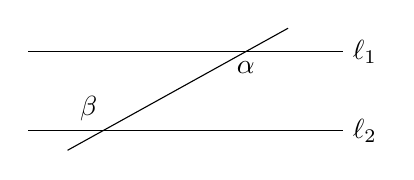
\begin{tikzpicture}
    \coordinate (A) at (0,1);
    \coordinate (B) at (4,1);
    \coordinate (C) at (0,0);
    \coordinate (D) at (4,0);
    \coordinate (E) at (0.5,-0.25);
    \coordinate (F) at (3.3,1.3);

\draw (A) -- (B) node[right] {$\ell_1$};
\draw (C) -- (D) node[right] {$\ell_2$};
\draw (E) -- (F);
\node at (3,1) [below left] {$\alpha$};
\node at (1,0) [above left] {$\beta$};
  \end{tikzpicture}
\end{center}
\end{lemma}
\begin{proof}[Skisse av bevis:]
Tegn en normal fra $\alpha$ ned til $\ell_2$. Siden $\ell_1,\ell_2$ er parallelle, får vi tok 90-gradersvinkler. Bruk nå at vinkelsummen er $180$ til å utlede at $\alpha=\beta$.
\end{proof}

Tilbake til løsningen av oppgaven. Siden $AD$ og $FC$ er parallelle, og $DB$ skjærer begge, får vi at vinklene $\angle CDA$ og $\angle BCF$ er like. I tillegg er $\angle FAD=\angle BFC$. Det følger at trekantene $\triangle ABD$ og $\triangle FBC$ er formlike.

På samme viset finner vi at $\triangle AFC$ er formlik med $\triangle ABE$ og at $\triangle ADC$ er formlik med $\triangle BEC$.

Vi får dermed følgende liste med likheter:
\begin{itemize}
\item $\frac{AF}{AB}=\frac{AC}{AE}=\frac{CF}{EB}$.
\item $\frac{AB}{FB}=\frac{BD}{BC}=\frac{DA}{CF}$.
\item $\frac{EB}{AD}=\frac{BC}{DC}=\frac{CE}{CA}$.
\end{itemize}
Ganger vi likhet nummer $1$ og $2$ sammen, får vi at
$$
\frac{AF}{FB} = \frac{CF \cdot DA}{EB \cdot CF} = \frac{DA}{EB}.
$$
Tilsvarende får vi at
$$
\frac{BD}{DC} = \frac{EB}{CF}  \qquad \frac{CE}{EA}=\frac{CF}{AD}.
$$
Ganger vi alle venstresidene sammen får vi forholdet vi var interessert i, mens ganger vi alle høyresidene sammen, får vi $1$. 

Vi har ikke brukt fortegnsmål her. Men observer at for punktene $D,E,F$ vil alltid $2$ ligge utenfor trekanten, og én på en av sidene (for å overbevise deg om dette: forestill deg at du vrir på linja gjennom $A$. Med en gang $D$ forlater linjestykket $BC$ vil $E$ eller $F$ komme på innsiden av trekanten). Dermed er fortegnet alltid positivt.

Og vi er ferdige.
  \begin{figure}
\centering
\definecolor{uuuuuu}{rgb}{0.266666666667,0.266666666667,0.266666666667}
\definecolor{zzttqq}{rgb}{0.6,0.2,0.}
\definecolor{qqqqff}{rgb}{0.,0.,1.}
\begin{tikzpicture}[line cap=round,line join=round,>=triangle 45,x=0.7cm,y=0.7cm]
\clip(-3.57640641535,-3.8197381551) rectangle (15.5370698726,8.33553493136);
\fill[color=zzttqq,fill=zzttqq,fill opacity=0.1] (4.02871400655,2.20332656263) -- (1.59569473278,-0.090663038361) -- (9.93747510001,-0.46140883246) -- cycle;
\draw [color=zzttqq] (4.02871400655,2.20332656263)-- (1.59569473278,-0.090663038361);
\draw [color=zzttqq] (1.59569473278,-0.090663038361)-- (9.93747510001,-0.46140883246);
\draw [color=zzttqq] (9.93747510001,-0.46140883246)-- (4.02871400655,2.20332656263);
\draw [domain=-3.57640641535:15.5370698726] plot(\x,{(-3.62624835225--2.28888616832*\x)/-0.288047377838});
\draw [domain=-3.57640641535:15.5370698726] plot(\x,{(-9.85593020459--2.28888616832*\x)/-0.288047377838});
\draw [domain=-3.57640641535:15.5370698726] plot(\x,{(-22.6128417001--2.28888616832*\x)/-0.288047377838});
\draw [domain=-3.57640641535:15.5370698726] plot(\x,{(-0.164694042589-0.370745794099*\x)/8.34178036723});
\draw [domain=-3.57640641535:15.5370698726] plot(\x,{(-23.7543870794--2.66473539509*\x)/-5.90876109345});
\draw [domain=-3.57640641535:15.5370698726] plot(\x,{(--3.8810920431-2.29398960099*\x)/-2.43301927377});
\begin{scriptsize}
\draw [fill=qqqqff] (4.02871400655,2.20332656263) circle (1.5pt);
\draw[color=qqqqff] (4.14150135403,2.4478245301) node {$A$};
\draw [fill=qqqqff] (1.59569473278,-0.090663038361) circle (1.5pt);
\draw[color=qqqqff] (1.72425954706,0.151444813488) node {$B$};
\draw [fill=qqqqff] (9.93747510001,-0.46140883246) circle (1.5pt);
\draw[color=qqqqff] (10.0637437811,-0.211141457557) node {$C$};
\draw [fill=uuuuuu] (1.14324272562,3.50461753246) circle (1.5pt);
\draw[color=uuuuuu] (1.25807719858,3.74277549812) node {$E$};
\draw [fill=uuuuuu] (4.33271220705,-0.21230825944) circle (1.5pt);
\draw[color=uuuuuu] (4.45228958635,0.0305827231399) node {$D$};
\draw [fill=uuuuuu] (9.01096065703,6.90087340451) circle (1.5pt);
\draw[color=uuuuuu] (9.06231503249,7.4377022602) node {$F$};
\end{scriptsize}
\end{tikzpicture}
    \caption{Oppgave 3.}
    
  \end{figure}
\end{losn}

\begin{oppg}
 Bruk Cevas setning til å vise at
 \begin{enumerate}[a)]
 \item  Høydene i en trekant er konkurrente.
 \item Medianene i en trekant er konkurrente.
 \item Vinklenes halveringslinjer i en trekant er konkurrente.
 \end{enumerate}
\end{oppg}
\begin{losn}
Vi gjør først a) og går rett på sak. Trekantene $\triangle BCF$ og $\triangle BDA$ er formlike, siden begge har vinkelen $\angle DBA$ og har en $90$-gradersvinkel. Dermed får vi at
$$
\frac{AB}{BC}=\frac{BD}{BF}=\frac{AD}{CF}.
$$
Tilsvarende får vi at trekantene $\triangle CAD$ og $\triangle BCE$ er formlike. Og at $\triangle ABE$ er formlik med $ACF$. Dermed får vi:
\begin{align*}
 \frac{CB}{CA} &= \frac{BE}{AD}= \frac{EC}{DC} \\
 \frac{AC}{AB} &= \frac{CF}{BE} = \frac{FA}{EA}.
\end{align*}

Ganger vi sammen nummer én og nummer tre, får vi at 
$$
\frac{AF}{FB} = \frac{AC}{BC}\cdot \frac{EA}{BD}.
$$
Ganger vi sammen én og to, får vi:
$$
\frac{BD}{DC} = \frac{AB}{CA} \cdot \frac{BF}{EC}
$$
Ganger vi sammen to og tre får vi:
$$
\frac{CE}{EA} = \frac{CB}{AB} \cdot \frac{DC}{FA}.
$$
Dermed blir Ceva-uttrykket:
$$
\frac{AF}{FB} \cdot \frac{BD}{DC} \frac{CE}{EA} = 1 pga kansellering [...]
$$

b) er triviell ($AF=BF$ osv per definisjon av median)

c) Dette følger fra setningen om halveringslinjer sammen med Ceva. (merk at vi ikke trenger sinus-setningen som er hint i oppgaven) 


  \begin{figure}
\centering
    \definecolor{uuuuuu}{rgb}{0.266666666667,0.266666666667,0.266666666667}
\definecolor{zzttqq}{rgb}{0.6,0.2,0.}
\definecolor{qqqqff}{rgb}{0.,0.,1.}
\begin{tikzpicture}[line cap=round,line join=round,>=triangle 45,x=0.7cm,y=0.7cm]
\clip(-4.3,-8.24) rectangle (19.92,6.3);
\fill[color=zzttqq,fill=zzttqq,fill opacity=0.1] (3.38,-4.02) -- (4.56,2.7) -- (11.48,-2.5) -- cycle;
\draw [color=zzttqq] (3.38,-4.02)-- (4.56,2.7);
\draw [color=zzttqq] (4.56,2.7)-- (11.48,-2.5);
\draw [color=zzttqq] (11.48,-2.5)-- (3.38,-4.02);
\draw [domain=-4.3:19.92] plot(\x,{(--27.4572-6.72*\x)/-1.18});
\draw [domain=-4.3:19.92] plot(\x,{(-37.6996--1.52*\x)/8.1});
\draw [domain=-4.3:19.92] plot(\x,{(-42.396--5.2*\x)/-6.92});
\draw [domain=-4.3:19.92] plot(\x,{(-41.04--8.1*\x)/-1.52});
\draw [domain=-4.3:19.92] plot(\x,{(--44.2936-6.92*\x)/-5.2});
\draw [domain=-4.3:19.92] plot(\x,{(-3.2536-1.18*\x)/6.72});
\begin{scriptsize}
\draw [fill=qqqqff] (4.56,2.7) circle (1.5pt);
\draw[color=qqqqff] (4.7,2.98) node {$A$};
\draw [fill=qqqqff] (3.38,-4.02) circle (1.5pt);
\draw[color=qqqqff] (3.54,-4.14) node {$B$};
\draw [fill=qqqqff] (11.48,-2.5) circle (1.5pt);
\draw[color=qqqqff] (11.62,-2.22) node {$C$};
\draw [fill=uuuuuu] (5.73800201412,-3.57751073315) circle (1.5pt);
\draw[color=uuuuuu] (5.88,-3.3) node {$D$};
\draw [fill=uuuuuu] (7.03318072135,0.841540498409) circle (1.5pt);
\draw[color=uuuuuu] (6.94,1.22) node {$E$};
\draw [fill=uuuuuu] (3.88120367427,-1.16568754995) circle (1.5pt);
\draw[color=uuuuuu] (4.08,-0.88) node {$F$};
\end{scriptsize}
\end{tikzpicture}
    \caption{Oppgave x}
    
  \end{figure}
\end{losn}

\end{document}
